
%% bare_conf.tex
%% V1.4b
%% 2015/08/26
%% by Michael Shell
%% See:
%% http://www.michaelshell.org/
%% for current contact information.
%%
%% This is a skeleton file demonstrating the use of IEEEtran.cls
%% (requires IEEEtran.cls version 1.8b or later) with an IEEE
%% conference paper.
%%
%% Support sites:
%% http://www.michaelshell.org/tex/ieeetran/
%% http://www.ctan.org/pkg/ieeetran
%% and
%% http://www.ieee.org/

%%*************************************************************************
%% Legal Notice:
%% This code is offered as-is without any warranty either expressed or
%% implied; without even the implied warranty of MERCHANTABILITY or
%% FITNESS FOR A PARTICULAR PURPOSE! 
%% User assumes all risk.
%% In no event shall the IEEE or any contributor to this code be liable for
%% any damages or losses, including, but not limited to, incidental,
%% consequential, or any other damages, resulting from the use or misuse
%% of any information contained here.
%%
%% All comments are the opinions of their respective authors and are not
%% necessarily endorsed by the IEEE.
%%
%% This work is distributed under the LaTeX Project Public License (LPPL)
%% ( http://www.latex-project.org/ ) version 1.3, and may be freely used,
%% distributed and modified. A copy of the LPPL, version 1.3, is included
%% in the base LaTeX documentation of all distributions of LaTeX released
%% 2003/12/01 or later.
%% Retain all contribution notices and credits.
%% ** Modified files should be clearly indicated as such, including  **
%% ** renaming them and changing author support contact information. **
%%*************************************************************************


% *** Authors should verify (and, if needed, correct) their LaTeX system  ***
% *** with the testflow diagnostic prior to trusting their LaTeX platform ***
% *** with production work. The IEEE's font choices and paper sizes can   ***
% *** trigger bugs that do not appear when using other class files.       ***                          ***
% The testflow support page is at:
% http://www.michaelshell.org/tex/testflow/



\documentclass[conference]{IEEEtran}
% Some Computer Society conferences also require the compsoc mode option,
% but others use the standard conference format.
%
% If IEEEtran.cls has not been installed into the LaTeX system files,
% manually specify the path to it like:
% \documentclass[conference]{../sty/IEEEtran}





% Some very useful LaTeX packages include:
% (uncomment the ones you want to load)


% *** MISC UTILITY PACKAGES ***
%
%\usepackage{ifpdf}
% Heiko Oberdiek's ifpdf.sty is very useful if you need conditional
% compilation based on whether the output is pdf or dvi.
% usage:
% \ifpdf
%   % pdf code
% \else
%   % dvi code
% \fi
% The latest version of ifpdf.sty can be obtained from:
% http://www.ctan.org/pkg/ifpdf
% Also, note that IEEEtran.cls V1.7 and later provides a builtin
% \ifCLASSINFOpdf conditional that works the same way.
% When switching from latex to pdflatex and vice-versa, the compiler may
% have to be run twice to clear warning/error messages.






% *** CITATION PACKAGES ***
%
%\usepackage{cite}
% cite.sty was written by Donald Arseneau
% V1.6 and later of IEEEtran pre-defines the format of the cite.sty package
% \cite{} output to follow that of the IEEE. Loading the cite package will
% result in citation numbers being automatically sorted and properly
% "compressed/ranged". e.g., [1], [9], [2], [7], [5], [6] without using
% cite.sty will become [1], [2], [5]--[7], [9] using cite.sty. cite.sty's
% \cite will automatically add leading space, if needed. Use cite.sty's
% noadjust option (cite.sty V3.8 and later) if you want to turn this off
% such as if a citation ever needs to be enclosed in parenthesis.
% cite.sty is already installed on most LaTeX systems. Be sure and use
% version 5.0 (2009-03-20) and later if using hyperref.sty.
% The latest version can be obtained at:
% http://www.ctan.org/pkg/cite
% The documentation is contained in the cite.sty file itself.






% *** GRAPHICS RELATED PACKAGES ***
%
\ifCLASSINFOpdf
  % \usepackage[pdftex]{graphicx}
  % declare the path(s) where your graphic files are
  % \graphicspath{{../pdf/}{../jpeg/}}
  % and their extensions so you won't have to specify these with
  % every instance of \includegraphics
  % \DeclareGraphicsExtensions{.pdf,.jpeg,.png}
\else
  % or other class option (dvipsone, dvipdf, if not using dvips). graphicx
  % will default to the driver specified in the system graphics.cfg if no
  % driver is specified.
  % \usepackage[dvips]{graphicx}
  % declare the path(s) where your graphic files are
  % \graphicspath{{../eps/}}
  % and their extensions so you won't have to specify these with
  % every instance of \includegraphics
  % \DeclareGraphicsExtensions{.eps}
\fi
% graphicx was written by David Carlisle and Sebastian Rahtz. It is
% required if you want graphics, photos, etc. graphicx.sty is already
% installed on most LaTeX systems. The latest version and documentation
% can be obtained at: 
% http://www.ctan.org/pkg/graphicx
% Another good source of documentation is "Using Imported Graphics in
% LaTeX2e" by Keith Reckdahl which can be found at:
% http://www.ctan.org/pkg/epslatex
%
% latex, and pdflatex in dvi mode, support graphics in encapsulated
% postscript (.eps) format. pdflatex in pdf mode supports graphics
% in .pdf, .jpeg, .png and .mps (metapost) formats. Users should ensure
% that all non-photo figures use a vector format (.eps, .pdf, .mps) and
% not a bitmapped formats (.jpeg, .png). The IEEE frowns on bitmapped formats
% which can result in "jaggedy"/blurry rendering of lines and letters as
% well as large increases in file sizes.
%
% You can find documentation about the pdfTeX application at:
% http://www.tug.org/applications/pdftex





% *** MATH PACKAGES ***
%
\usepackage{amsmath}
% A popular package from the American Mathematical Society that provides
% many useful and powerful commands for dealing with mathematics.
%
% Note that the amsmath package sets \interdisplaylinepenalty to 10000
% thus preventing page breaks from occurring within multiline equations. Use:
%\interdisplaylinepenalty=2500
% after loading amsmath to restore such page breaks as IEEEtran.cls normally
% does. amsmath.sty is already installed on most LaTeX systems. The latest
% version and documentation can be obtained at:
% http://www.ctan.org/pkg/amsmath





% *** SPECIALIZED LIST PACKAGES ***
%
%\usepackage{algorithmic}
% algorithmic.sty was written by Peter Williams and Rogerio Brito.
% This package provides an algorithmic environment fo describing algorithms.
% You can use the algorithmic environment in-text or within a figure
% environment to provide for a floating algorithm. Do NOT use the algorithm
% floating environment provided by algorithm.sty (by the same authors) or
% algorithm2e.sty (by Christophe Fiorio) as the IEEE does not use dedicated
% algorithm float types and packages that provide these will not provide
% correct IEEE style captions. The latest version and documentation of
% algorithmic.sty can be obtained at:
% http://www.ctan.org/pkg/algorithms
% Also of interest may be the (relatively newer and more customizable)
% algorithmicx.sty package by Szasz Janos:
% http://www.ctan.org/pkg/algorithmicx




% *** ALIGNMENT PACKAGES ***
%
%\usepackage{array}
% Frank Mittelbach's and David Carlisle's array.sty patches and improves
% the standard LaTeX2e array and tabular environments to provide better
% appearance and additional user controls. As the default LaTeX2e table
% generation code is lacking to the point of almost being broken with
% respect to the quality of the end results, all users are strongly
% advised to use an enhanced (at the very least that provided by array.sty)
% set of table tools. array.sty is already installed on most systems. The
% latest version and documentation can be obtained at:
% http://www.ctan.org/pkg/array


% IEEEtran contains the IEEEeqnarray family of commands that can be used to
% generate multiline equations as well as matrices, tables, etc., of high
% quality.




% *** SUBFIGURE PACKAGES ***
%\ifCLASSOPTIONcompsoc
%  \usepackage[caption=false,font=normalsize,labelfont=sf,textfont=sf]{subfig}
%\else
%  \usepackage[caption=false,font=footnotesize]{subfig}
%\fi
% subfig.sty, written by Steven Douglas Cochran, is the modern replacement
% for subfigure.sty, the latter of which is no longer maintained and is
% incompatible with some LaTeX packages including fixltx2e. However,
% subfig.sty requires and automatically loads Axel Sommerfeldt's caption.sty
% which will override IEEEtran.cls' handling of captions and this will result
% in non-IEEE style figure/table captions. To prevent this problem, be sure
% and invoke subfig.sty's "caption=false" package option (available since
% subfig.sty version 1.3, 2005/06/28) as this is will preserve IEEEtran.cls
% handling of captions.
% Note that the Computer Society format requires a larger sans serif font
% than the serif footnote size font used in traditional IEEE formatting
% and thus the need to invoke different subfig.sty package options depending
% on whether compsoc mode has been enabled.
%
% The latest version and documentation of subfig.sty can be obtained at:
% http://www.ctan.org/pkg/subfig




% *** FLOAT PACKAGES ***
%
%\usepackage{fixltx2e}
% fixltx2e, the successor to the earlier fix2col.sty, was written by
% Frank Mittelbach and David Carlisle. This package corrects a few problems
% in the LaTeX2e kernel, the most notable of which is that in current
% LaTeX2e releases, the ordering of single and double column floats is not
% guaranteed to be preserved. Thus, an unpatched LaTeX2e can allow a
% single column figure to be placed prior to an earlier double column
% figure.
% Be aware that LaTeX2e kernels dated 2015 and later have fixltx2e.sty's
% corrections already built into the system in which case a warning will
% be issued if an attempt is made to load fixltx2e.sty as it is no longer
% needed.
% The latest version and documentation can be found at:
% http://www.ctan.org/pkg/fixltx2e


%\usepackage{stfloats}
% stfloats.sty was written by Sigitas Tolusis. This package gives LaTeX2e
% the ability to do double column floats at the bottom of the page as well
% as the top. (e.g., "\begin{figure*}[!b]" is not normally possible in
% LaTeX2e). It also provides a command:
%\fnbelowfloat
% to enable the placement of footnotes below bottom floats (the standard
% LaTeX2e kernel puts them above bottom floats). This is an invasive package
% which rewrites many portions of the LaTeX2e float routines. It may not work
% with other packages that modify the LaTeX2e float routines. The latest
% version and documentation can be obtained at:
% http://www.ctan.org/pkg/stfloats
% Do not use the stfloats baselinefloat ability as the IEEE does not allow
% \baselineskip to stretch. Authors submitting work to the IEEE should note
% that the IEEE rarely uses double column equations and that authors should try
% to avoid such use. Do not be tempted to use the cuted.sty or midfloat.sty
% packages (also by Sigitas Tolusis) as the IEEE does not format its papers in
% such ways.
% Do not attempt to use stfloats with fixltx2e as they are incompatible.
% Instead, use Morten Hogholm'a dblfloatfix which combines the features
% of both fixltx2e and stfloats:
%
% \usepackage{dblfloatfix}
% The latest version can be found at:
% http://www.ctan.org/pkg/dblfloatfix




% *** PDF, URL AND HYPERLINK PACKAGES ***
%
%\usepackage{url}
% url.sty was written by Donald Arseneau. It provides better support for
% handling and breaking URLs. url.sty is already installed on most LaTeX
% systems. The latest version and documentation can be obtained at:
% http://www.ctan.org/pkg/url
% Basically, \url{my_url_here}.




% *** Do not adjust lengths that control margins, column widths, etc. ***
% *** Do not use packages that alter fonts (such as pslatex).         ***
% There should be no need to do such things with IEEEtran.cls V1.6 and later.
% (Unless specifically asked to do so by the journal or conference you plan
% to submit to, of course. )

\usepackage{graphicx}
\usepackage[labelfont=bf]{caption}
%\usepackage[superscript,nomove]{cite}
\usepackage{color}
\usepackage{wrapfig,booktabs}
% correct bad hyphenation here
\hyphenation{op-tical net-works semi-conduc-tor}


\begin{document}
%
% paper title
% Titles are generally capitalized except for words such as a, an, and, as,
% at, but, by, for, in, nor, of, on, or, the, to and up, which are usually
% not capitalized unless they are the first or last word of the title.
% Linebreaks \\ can be used within to get better formatting as desired.
% Do not put math or special symbols in the title.
\title{Did you take the pill? - Stacked Ensemble of CNNs for Identifying Mentions of Personal Intake of Medicine in Twitter}


% author names and affiliations
% use a multiple column layout for up to three different
% affiliations
\author{\IEEEauthorblockN{Jasper Friedrichs}
\IEEEauthorblockA{Lyft, Palo Alto, USA\\
Email: jasper.friedrichs@gmail.com }
\and
\IEEEauthorblockN{Debanjan Mahata}
\IEEEauthorblockA{Bloomberg L.P., New York, USA\\
Email: dmahata@bloomberg.net}
\and
\IEEEauthorblockN{Rajiv Ratn Shah}
\IEEEauthorblockA{Singapore Management University, Singapore\\
Email: rajivshah@smu.edu.sg}
\and
\IEEEauthorblockN{Jing Jiang}
\IEEEauthorblockA{Singapore Management University, Singapore\\
Emai: jingjiang@smu.edu.sg}}

% conference papers do not typically use \thanks and this command
% is locked out in conference mode. If really needed, such as for
% the acknowledgment of grants, issue a \IEEEoverridecommandlockouts
% after \documentclass

% for over three affiliations, or if they all won't fit within the width
% of the page, use this alternative format:
% 
%\author{\IEEEauthorblockN{Michael Shell\IEEEauthorrefmark{1},
%Homer Simpson\IEEEauthorrefmark{2},
%James Kirk\IEEEauthorrefmark{3}, 
%Montgomery Scott\IEEEauthorrefmark{3} and
%Eldon Tyrell\IEEEauthorrefmark{4}}
%\IEEEauthorblockA{\IEEEauthorrefmark{1}School of Electrical and Computer Engineering\\
%Georgia Institute of Technology,
%Atlanta, Georgia 30332--0250\\ Email: see http://www.michaelshell.org/contact.html}
%\IEEEauthorblockA{\IEEEauthorrefmark{2}Twentieth Century Fox, Springfield, USA\\
%Email: homer@thesimpsons.com}
%\IEEEauthorblockA{\IEEEauthorrefmark{3}Starfleet Academy, San Francisco, California 96678-2391\\
%Telephone: (800) 555--1212, Fax: (888) 555--1212}
%\IEEEauthorblockA{\IEEEauthorrefmark{4}Tyrell Inc., 123 Replicant Street, Los Angeles, California 90210--4321}}




% use for special paper notices
%\IEEEspecialpapernotice{(Invited Paper)}




% make the title area
\maketitle

% As a general rule, do not put math, special symbols or citations
% in the abstract
\begin{abstract}
Mining social media messages such as tweets, articles, and Facebook
posts for health and drug related information has received significant interest in pharmacovigilance research. Social media sites (e.g., Twitter), have been used for monitoring drug abuse, adverse reactions of drug usage and analyzing expression of sentiments related to drugs. Most of these studies are based on aggregated results from a large population rather than specific sets of individuals. In order to conduct studies at an individual level or specific cohorts, identifying posts mentioning intake of medicine by the user is necessary. Towards this objective we develop a classifier for identifying mentions of personal intake of medicine in tweets. We train a
stacked ensemble of shallow convolutional neural network (CNN) models on an annotated dataset. We use random search for tuning the hyper-parameters of the CNN models and present an ensemble of best models for the prediction task. Our system produces state-of-the-art result, with a micro-averaged F-score of 0.693. 
\end{abstract}

% no keywords




% For peer review papers, you can put extra information on the cover
% page as needed:
% \ifCLASSOPTIONpeerreview
% \begin{center} \bfseries EDICS Category: 3-BBND \end{center}
% \fi
%
% For peerreview papers, this IEEEtran command inserts a page break and
% creates the second title. It will be ignored for other modes.
\IEEEpeerreviewmaketitle



\section{Introduction}
Social media has become an ubiquitous source of information for a variety of topics. Right from information related to daily events, personal rants, to expressions of intake of medicine and adverse drug reactions, are readily available in publicly accessible social media channels such as Twitter\footnote{http://twitter.com}, DailyStrength\footnote{https://www.dailystrength.org/}, MedHelp\footnote{http://www.medhelp.org/}, among others. Huge amounts of data made available on these platforms have become an useful resource for conducting public health monitoring and surveillance, commonly known as pharmacovigilance \cite{harmark2008pharmacovigilance}. The work presented in this paper aims at identifying intake of personal medication expressed by an user in Twitter. The broader perspective of such a system is to aid in developing automated methods for performing pharmacovigilance activities in social media, and to study the effects of medicine on an individual as well as specific cohorts \cite{klein2017detecting}.

Substantial attempts have been made to mine social media content in order to identify adverse drug reactions \cite{nikfarjam2015pharmacovigilance}, abuse \cite{hanson2013tweaking}, and user sentiment \cite{korkontzelos2016analysis}, from posts mentioning medications. However, all these studies are based on aggregated results from large set of content that mentions a medicine/drug, without taking into account whether the user has actually consumed the medicine/drug. Without this knowledge, a true assessment of the effects of medication intake in general and how it affects a specific group of users cannot be done. In order to leverage social media data for studying targeted groups and to do a true assessment of the effects of medication intake, it is necessary to develop systems that can automatically distinguish posts that expresses personal intake of medicine from those that do not. In this work we only concentrate on Twitter as the social media channel for performing such a task.

The key to the process of identifying tweets mentioning personal intake of medicine and to draw insights from them is to build accurate text classification systems. The effectiveness of developing classifiers has already been shown to be useful in identifying adverse drug reactions expressed in Twitter \cite{nikfarjam2015pharmacovigilance}. However, mining social media posts comes with unique challenges. Microblogging websites like Twitter pose challenges for automated information mining tools and techniques due to their brevity, noisiness, idiosyncratic language, unusual structure and ambiguous representation of discourse. Information extraction tasks using state-of-the-art natural language processing techniques, often give poor results for tweets. Abundance of link farms, unwanted promotional posts, and nepotistic relationships between content creates additional challenges \cite{mahata2015chirps}.

The main objective of the task presented in this paper is to categorize short colloquial tweets into one of the three categories, 
\begin{enumerate}
\item \textit{\textbf{personal medication intake} (Class 1)} - tweets in which the user clearly expresses a personal medication in-take/consumption ( e.g. \textit{I had the worst headache ever and I just took an \@AdvilRelief \#advil and now I feel so much better thank}).
\item \textit{\textbf{possible medication intake} (Class 2)} - tweets that are ambiguous but suggest that the user may have taken the medication (e.g. \textit{I should have taken advil on friday then i might have actully had an amazing weekend.. instead of throwing up 20 times a day \#advil, not this time})
\item \textit{\textbf{non-intake} (Class 3)} - tweets that mention medication names but do not indicate personal intake (e.g. \textit{Understand the causes and managing \#Migraine Madness \#aspirin \#diet \#botox \#advil \#relpax \#headache}). 
\end{enumerate}

Towards the above goal, we design and implement a deep learning classifier - \textit{Stacked Ensemble of Shallow Convolutional Neural Networks} (Section \ref{stackedCNN}), trained on an annotated dataset provided at SMM4H-2017 shared task workshop\footnote{https://healthlanguageprocessing.org/sharedtask2/}. We compare the results of our classification system with other classifiers that participate in the shared task and get state-of-the-art results, with a micro-averaged F-score of 0.693 for Class 1 and 2. We submitted our system (\textit{InfyNLP}) at the workshop and was ranked first amongst 26 submissions \cite{sarker1overview, infynlpsmm4h}. In this paper, we intend to elaborately discuss and present our submitted system as well as our model choices and learnings.

Next, we present work related and relevant to the scope of this paper.

\section{Related Work}

Pharmacovigilance is the branch of pharmacological sciences that deals with drug safety. It studies
the collection, detection, monitoring, assessment, and prevention of harmful effects with
pharmaceutical products. Mining social media messages such as tweets, blog articles, and Facebook
posts for health and drug related information has received significant interest in
pharmacovigilance research as people tend to share their daily activities on social media.
Since pharmacovigilance heavily focuses on adverse drug reactions, it necessitates an automatic
detection of the personal intake of medicine by sensing the social media to build smart
health-care applications. Thus, developing automated classification models for identifying
messages (e.g., tweets) containing description of personal intake of medicine is a pragmatic
step towards the automation of Pharmacovigilance. Cramer~\emph{et al.}~\cite{cramer1989often} 
found that as we increase the number of dosages of medicines (say from one to four times) in 
a day, compliance rate decreases. Thus, several research work~\cite{harmark2008pharmacovigilance, saparova2012motivating, cambria2012sentic} 
discussed and explored different healthcare problems through advanced technologies. 
In this section, we provide a brief literature review on this problem.

Due to active participation of users on social media, it is now feasible
to classify latent user attributes (\emph{e.g.}, gender, age, regional origin,
and political orientation) in social media such as Twitter~\cite{rao2010classifying}.
Research studies in last few years indicate that social media is heavily used
in building healthcare applications~\cite{grajales2014social, Sarker2016, rosenthal2017semeval}.
Sarker~\emph{et al.}~\cite{sarker2015utilizing} presented a review of pharmacovigilance techniques from
social media data and discussed a possible pathway for automated pharmacovigilance research.

Deep learning techniques have yielded immense success in computer vision, natural 
language processing, speech processing, machine translation, and 
healthcare~\cite{kim2014convolutional, liang2014deep, shin2016lexicon, denkowski2017stronger}. 
However, training deep neural networks to obtain good models is not easy and depends on 
determining hyper-parameters optimally~\cite{glorot2010understanding}. 
Bergstra~\emph{et al.}~\cite{bergstra2012random} performed random search for hyper-parameter 
optimization. Moreover, Lim~\emph{et al.}~\cite{lin2014user} used deep neural network 
techniques to detect user-level psychological stress from social media. However, only
going deeper with convolutions does not lead to the best solution~\cite{szegedy2015going}. 
Recent studies such as Le~\emph{et al.}~\cite{le2017convolutional} explored 
shallow networks for text classification. They found that their shallow word models outperform 
deeper models. This encouraged us to use a shallow network in our proposed approach 
for identifying personal medication intake from Twitter.

%Recently, Klein~\emph{et al.}~\cite{klein2017detecting} presented an annotated corpus
%to train machine learning models to find whether a tweet with a mention of medication implies
%that the person (i.e, Twitterer) has taken that medication or not.

Often one solution to a complex problem does not fit to all scenarios~\cite{bell2010all}.
Thus, researchers use ensemble techniques to address such problems. Zhou~\emph{et al.}~\cite{zhou2002ensembling} presented a neural network ensemble and proposed, that many neural networks can be jointly used to solve a problem efficiently. 
For instance, Deng and Platt~\cite{deng2014ensemble} use an ensemble of deep learning models for speech 
recognition. Wang~\emph{et al.}~\cite{wang2008biomedical} presented \textit{ensemble of classifier} approaches 
for biomedical named entity recognition by combining \textit{generalized winnow}, 
\textit{conditional random fields}, \textit{support vector machine}, and \textit{maximum entropy} through three 
different strategies. Moreover, ensemble techniques have shown to perform well in 
biomedical entity extraction~\cite{ekbal2013stacked} and named entity 
recognition~\cite{sikdar2012differential, speck2014ensemble}. Furthermore, 
stacked ensemble techniques are very useful in different healthcare 
applications~\cite{dinakar2014stacked, speck2014ensemble}. A recent work~\cite{liu2016ensemble} proposed an ensemble of several classifiers that effectively distinguishes between adverse drug events (ADEs) and non-ADEs from  
informal text in social media. 

Our literature review confirms that leveraging social media data using ensemble and 
neural network techniques is very beneficial in healthcare applications. Thus, in order to solve the problem of identifying personal 
medication intake from Twitter, we train a stacked ensemble of shallow convolutional neural 
network (CNN) models on an annotated dataset. We use random 
search for tuning the hyper-parameters of the CNN and build an ensemble of best models that 
achieves state-of-the-art performance. 

\begin{figure*}[htbp]
	\centering
	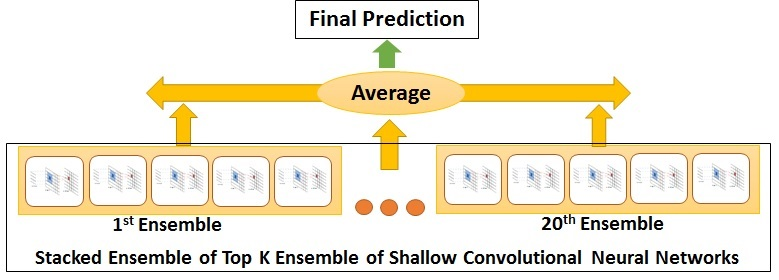
\includegraphics[width=12cm,height=10cm,keepaspectratio]{StackedCNN.jpg}
	\caption{A Stacked Ensemble of 100 (20 x 5) shallow convolutional neural networks.}
	\label{stackedcnn}
\end{figure*}


\section{Methodology}
Deep learning systems have recently shown to achieve top results in tasks related to natural language processing on tweets \cite{rosenthal2017semeval}. Historically, ensemble learning has proved to be very effective in most of the machine learning tasks including the famous winning solution of the Netflix Prize \cite{bell2010all}. Ensemble models can offer diversity over training data splits, random initialization of the same model or model architectures, and a combination of multiple average or low performing learners to produce a robust and high-performing learning model. A convolutional neural network (CNN) is a deep learning architecture, that has shown strong performance on sentence-level text classification \cite{kim2014convolutional}. Even fairly simple CNNs evaluate at a level of or even better than more complex deep learning architectures \cite{le2017convolutional}. Therefore, we design and implement a stacked ensemble of shallow convolutional neural networks (Figure 1) for solving the classification task presented in this paper. The main intuition behind developing such an ensemble was to take the best of both worlds. Next, we explain the architecture of stacked ensemble of CNNs that we train.


\subsection{Stacked Ensemble of Shallow Convolutional Neural Networks \label{stackedCNN}}
\textit{A Stacked Ensemble of Shallow Convolutional Neural Networks} is a large ensemble classifier comprising of smaller ensembles stacked over one another, with the underlying classifier being a standard shallow Convolutional Neural Network (CNN) model similar to that used in \cite{kim2014convolutional}. In order to train such an ensemble model we enlist the generic steps:
\begin{enumerate}
\item[Step 1] Train a shallow CNN model on each fold while performing \textit{c-fold} cross validation on the training dataset.
\item[Step 2] The output of each model trained on each fold is averaged to get the final output of an ensemble of $c$ CNN models ($ensemble_{i}^{output}$, Equation \ref{eq1}).
\item[Step 3] Train $n$ such ensembles as in Step 2. 
\item[Step 4] Sort the $n$ ensembles in terms of their performance on the metric suitable for the classification task. 
\item[Step 5]Choose top $K$ ensembles based on their performance on the training dataset to form the final stacked ensemble of $K$ CNN ensemble models.
\item[Step 5] The final output prediction ($stacked-ensemble^{output}$), is given by the average of the predictions made by each of the top $K$ ensembles (Equation \ref{eq2}).
\end{enumerate}


\begin{equation}
\label{eq1}
\begin{split}
ensemble_{i}^{output} = average(prediction_{1}, prediction_{2}, \\ ..., prediction_{c})
\end{split}
\end{equation}

\begin{equation}
\label{eq2}
\begin{split}
stacked-ensemble^{output} = average(ensemble_{top_{1}}^{output}, \\ ensemble_{top_{2}}^{output},..., ensemble_{top_{K}}^{output}), \\ \\
%s.t, \ \{ensemble_{top_{1}}^{output} > ensemble_{top_{2}}^{output} >... > \\ ensemble_{top_{K}}^{output}\}
\end{split}
\end{equation}

Figure \ref{stackedcnn}, shows a high level architecture of the final stacked ensemble of CNNs that we use in predicting the outcome of the task presented in this paper. We train a standard shallow CNN model, on each fold while performing 5-fold cross validation on our training dataset. We take the output prediction of each of these models trained on each fold and average them to create an ensemble of 5 models. We further train $20$ such ensembles. For the final output we sort the ensembles in order of their decreasing performance on the training dataset and take the $top \ k$ ensembles. We take the output of each ensemble and average them to create our stacked ensemble of shallow CNNs.  We call this architecture as a stacked ensemble as we stack one ensemble over another in order to create the final ensemble of models that we use for prediction. In general, we can take top K such ensembles and create a stacked ensemble of top K ensemble of shallow CNNs.

%\subsection{Random Search of Hyperparameters}
In order to get the best results from any classification model, hyperparameter tuning is a key step and CNNs are no exception. While the existing literature offers guidance on practical design decisions, identifying the best hyperparameters of a CNN requires experimentation. This requires evaluating trained models on a cross-validation dataset and choosing the best hyperparameters manually that produce best results. Automated hyperparameter searching methods like \textit{grid search}, \textit{random search}, and \textit{bayesian optimization} methods are also popularly used. In our presented system we use random search \cite{bergstra2012random}, to explore the hyperparameters of a shallow CNN architecture and form an ensemble of the best models, which we refer to as a stacked ensemble. Next, we share the detailed settings, output and analysis of our experiment.

\section{Experiment} 
In this section, we present the experiments that we perform on the dataset in order to achieve the task presented in this paper. We give an overview of the dataset on which we train our models, and discuss about the hyperparameter settings. Results of our experiments are presented accompanied by a discussion of 
\subsection{Dataset \label{dataset}}
The dataset used in this paper is publicly available and can be obtained from 2nd Social Media Mining for Health Applications Shared Task at AMIA 2017 website\footnote{https://healthlanguageprocessing.org/sharedtask2/}.
The organizers of the task provided 8000 annotated tweets as a training dataset and 2260 additional tweets as development dataset. We collected the tweets using the script provided along with the dataset, by querying Twitter’s API. However, we could not collect all the tweets as some of them were not available at the moment when we executed our collection process. Later, the organizers also shared the test dataset, that was used for calculating the final scores of the submitted models. The test dataset consisted 7513 tweets. A distribution of tweets provided for each class and the mapping of each class is shown in Table 1. It is to be noted over here that for training our models, we combine the training and development dataset provided and treat it as our training dataset, therefore learning our models using 9663 tweets with 5-fold cross validation.

\begin{table}[htbp]
\centering
\tabcolsep=0.10cm
\begin{tabular}{|l|l|l|l|l|}
\hline
 & \textbf{Class 1} & \textbf{Class 2} & \textbf{Class 3} & \textbf{Total} \\ \hline
\textbf{Train} & 1847 & 3027 & 4789 & 9663 \\ \hline
\textbf{Test} & 1731 & 2697 & 3085 & 7513 \\ \hline
\end{tabular}
\caption{Shared task data distribution. Class 1, 2 and 3 represents \textit{personal medication intake}, \textit{possible medication intake} and \textit{no medication intake}, respectively.}
\label{dataset}
\end{table}

\subsection{Data Preprocessing}
We use Spacy\footnote{https://spacy.io/}  for all our data preprocessing and cleaning activities. We do not remove stopwords. Each document in our training and test dataset is converted to a fixed size document of 47 words/tokens. We use two pre-trained word embeddings - godin \cite{godin2015multimedia} and shin \cite{shin2016lexicon}, shared by the authors. Each of these embeddings are of 400 dimensions. Each word in the input tweet is represented by its corresponding embedding vector, when present in the vocabulary of the model.

\begin{table}[htbp]
\centering
\tabcolsep=0.10cm
\begin{tabular}{|c|c|}
\hline
\textbf{Hyperparameter} & \textbf{Range} \\ \hline
\textit{\textbf{adam\_b2}} & 0.9, 0.999 \\ \hline
\textit{\textbf{n\_dense\_output}} & 100, 200, 300, 400 \\ \hline
\textit{\textbf{keep\_prob (dropout)}} & 0.4, 0.5, 0.6, 0.7, 0.8, 0.9 \\ \hline
\textit{\textbf{batch\_size}} & 50, 100, 150 \\ \hline
\textit{\textbf{learning\_rate}} & 0.0001, 0.001 \\ \hline
\textit{\textbf{word\_embedding}} & godin \cite{godin2015multimedia}, shin \cite{shin2016lexicon} \\ \hline
\textit{\textbf{n\_filters}} & 100, 200, 300, 400 \\ \hline
\textit{\textbf{filter\_sizes}} & \multicolumn{1}{l|}{\begin{tabular}[c]{@{}l@{}}{[}1,2,3,4,5{]}, {[}2,3,4,5,6{]}, \\ {[}3,4,5,6,7{]}, {[}1,2,2,2,3{]},\\ {[}2,3,3,3,4{]}, {[}3,4,4,4,5{]},\\ {[}4,5,5,5,6{]}\end{tabular}} \\ \hline
\end{tabular}
\caption{Hyperparameter ranges used for random search permutations.}
\label{table_hyperparameters}
\end{table}

\subsection{Hyperparameter Settings for CNNS}
We use Xavier weight initialization scheme \cite{glorot2010understanding}, for initializing the weights of the CNNs. Adam \cite{kingma2014adam} with two annealing restarts has been shown to work faster and perform better than SGD in other NLP tasks \cite{denkowski2017stronger}. Therefore, we use the same as our optimization algorithm. We use five filters with varying filter sizes in the convolution layer and use dropout during the training process. The models are implemented using TensorFlow\footnote{https://www.tensorflow.org/}. The entire ranges of the hyperparameters that we give to our random search procedure is shown in Table \ref{table_hyperparameters}. The word embedding model to be used during training is also treated as a hyperparameter.

\begin{figure*}[htbp]
	\centering
	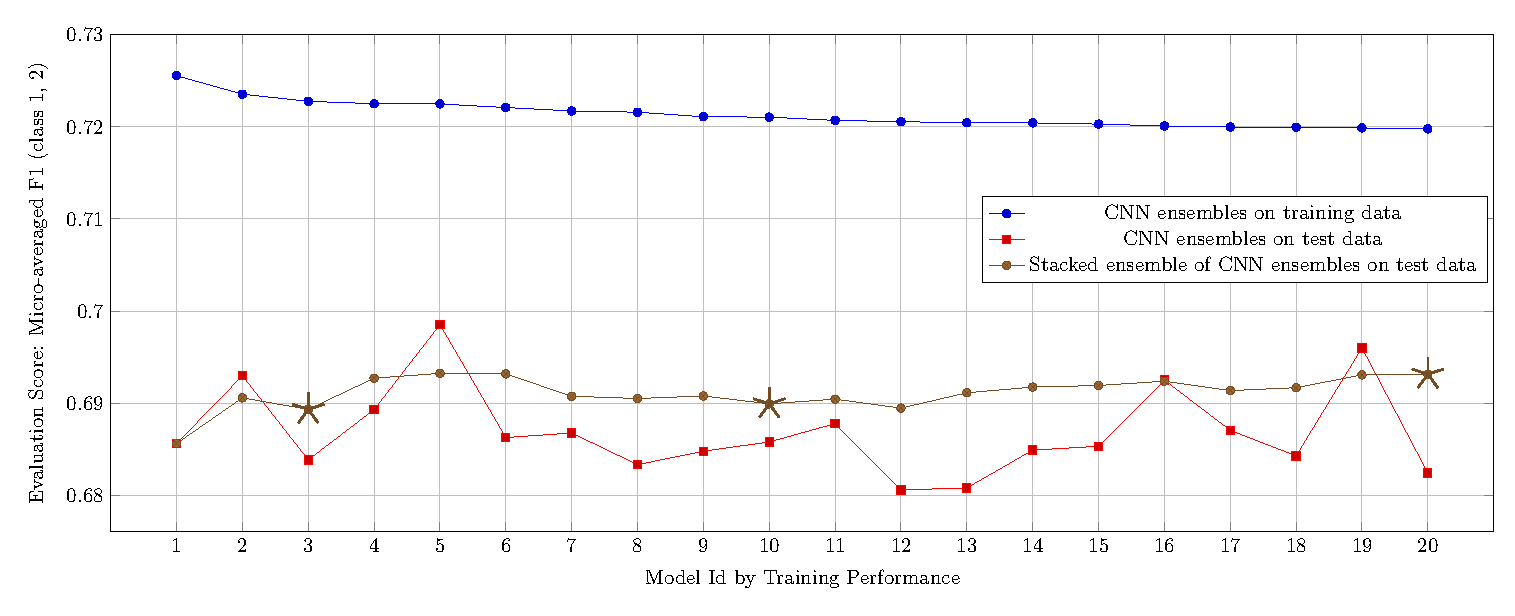
\includegraphics[scale=0.65]{ensemble_plot.pdf}
	\caption{Individual 5-fold data ensemble and collective parameter ensemble (stacked ensemble) results for top 20 random search models. Models are sorted from left to right by decreasing 5-fold cross validation results. }
	\label{plot_ensemble_eval}
\end{figure*}

\begin{figure*}[htbp]
	\centering
	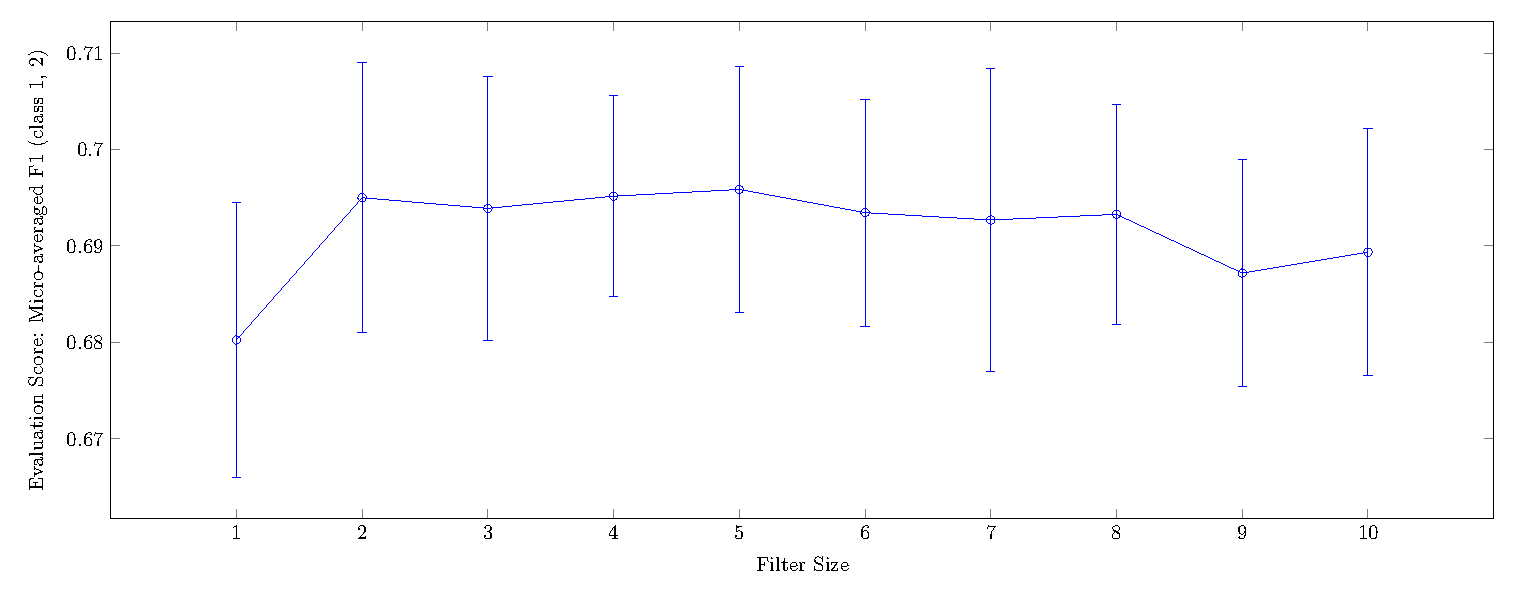
\includegraphics[scale=0.65]{filter_plot.pdf}
	\caption{Individual 5-fold data ensemble and collective parameter ensemble (stacked ensemble) results for top 20 random search models. Models are sorted from left to right by decreasing 5-fold cross validation results. }
	\label{plot_ensemble_eval}
\end{figure*}

\subsection{Results \label{results}}

\begin{equation}
Precision_{1 + 2} = \frac{TP_{1} + TP_{2}}{TP_{1} + FP_{1} + TP_{2} + FP_{2}}
\end{equation}

\begin{equation}
Recall_{1 + 2} = \frac{TP_{1} + TP_{2}}{TP_{1} + FN_{1} + TP_{2} + FN_{2}}
\end{equation}

\begin{equation}
F-Score_{1+2} = \frac{2*Precision_{1 + 2}*Recall_{1 + 2}}{Precision_{1 + 2} + Recall_{1 + 2}}
\end{equation}

\begin{table*}[htbp]
\centering
\tabcolsep=0.10cm
\begin{tabular}{clclllclllclccl}
\textbf{} &  & \textbf{Recall} & \textbf{} & \textbf{} &  & \textbf{Precision} & \textbf{} & \textbf{} &  & \textbf{F1} & \textbf{} & \textbf{Recall\_m} & \textbf{Precision\_m} & \textbf{F1\_m} \\ \hline
\multicolumn{1}{|c|}{} & \multicolumn{1}{c|}{\textbf{1}} & \multicolumn{1}{c|}{\textbf{2}} & \multicolumn{1}{c|}{\textbf{3}} & \multicolumn{1}{c|}{} & \multicolumn{1}{c|}{\textbf{1}} & \multicolumn{1}{c|}{\textbf{2}} & \multicolumn{1}{c|}{\textbf{3}} & \multicolumn{1}{c|}{} & \multicolumn{1}{c|}{\textbf{1}} & \multicolumn{1}{c|}{\textbf{2}} & \multicolumn{1}{c|}{\textbf{3}} & \multicolumn{1}{c|}{\textbf{}} & \multicolumn{1}{c|}{\textbf{}} & \multicolumn{1}{c|}{\textbf{}} \\ \hline
\multicolumn{1}{|c|}{\textit{\textbf{top 3}}} & \multicolumn{1}{l|}{0.696} & \multicolumn{1}{c|}{0.644} & \multicolumn{1}{l|}{0.842} & \multicolumn{1}{l|}{} & \multicolumn{1}{l|}{0.704} & \multicolumn{1}{c|}{0.725} & \multicolumn{1}{l|}{\textbf{0.763}} & \multicolumn{1}{l|}{} & \multicolumn{1}{l|}{0.700} & \multicolumn{1}{c|}{0.682} & \multicolumn{1}{l|}{0.800} & \multicolumn{1}{c|}{\textbf{0.664}} & \multicolumn{1}{c|}{0.716} & \multicolumn{1}{l|}{0.689} \\ \hline
\multicolumn{1}{|c|}{\textit{\textbf{top 10}}} & \multicolumn{1}{l|}{0.685} & \multicolumn{1}{c|}{0.646} & \multicolumn{1}{l|}{0.849} & \multicolumn{1}{l|}{} & \multicolumn{1}{l|}{0.709} & \multicolumn{1}{c|}{0.729} & \multicolumn{1}{l|}{0.758} & \multicolumn{1}{l|}{} & \multicolumn{1}{l|}{0.697} & \multicolumn{1}{c|}{0.685} & \multicolumn{1}{l|}{0.801} & \multicolumn{1}{c|}{0.661} & \multicolumn{1}{c|}{0.721} & \multicolumn{1}{l|}{0.690} \\ \hline
\multicolumn{1}{|c|}{\textit{\textbf{top 20}}} & \multicolumn{1}{l|}{\textbf{0.690}} & \multicolumn{1}{c|}{\textbf{0.648}} & \multicolumn{1}{l|}{\textbf{0.853}} & \multicolumn{1}{l|}{} & \multicolumn{1}{l|}{\textbf{0.712}} & \multicolumn{1}{c|}{\textbf{0.733}} & \multicolumn{1}{l|}{0.761} & \multicolumn{1}{l|}{} & \multicolumn{1}{l|}{\textbf{0.701}} & \multicolumn{1}{c|}{\textbf{0.688}} & \multicolumn{1}{l|}{\textbf{0.804}} & \multicolumn{1}{c|}{\textbf{0.664}} & \multicolumn{1}{c|}{\textbf{0.725}} & \multicolumn{1}{l|}{\textbf{0.693$\ast$}} \\ \hline
\end{tabular}
\caption{Evaluation of ensembles on test data. \_m stands for micro average recall over class 1 and 2. $\ast$ marks the state-of-the-art micro averaged F1 on the task's dataset achieved by our best model.}
\label{table_ensemble_results}
\end{table*}

\begin{table}[]
\centering
\begin{tabular}{|c|c|c|c|}
\hline
\textbf{Systems} & \textbf{\begin{tabular}[c]{@{}c@{}}Micro-averaged\\ Precision\\ Class 1 and 2\end{tabular}} & \textbf{\begin{tabular}[c]{@{}c@{}}Micro-averaged\\ Recall\\  Class 1 and 2\end{tabular}} & \textbf{\begin{tabular}[c]{@{}c@{}}Micro-averaged\\ F-score \\ Class 1 and 2\end{tabular}} \\ \hline
\textbf{InfyNLP} & \textbf{0.725} & 0.664 & \textbf{0.693} \\ \hline
\textbf{UKNLP} & 0.701 & \textbf{0.677} & 0.689 \\ \hline
\textbf{NRC-Canada} & 0.704 & 0.635 & 0.668 \\ \hline
\textbf{TJIIP} & 0.654 & 0.664 & 0.659 \\ \hline
\textbf{CSaRus-CNN} & 0.709 & 0.604 & 0.652 \\ \hline
\end{tabular}
\caption{My caption}
\label{my-label}
\end{table}


An ensemble of five CNNs is trained during 5-fold cross-validation training performed on our combined training dataset along with random search on the hyperparameter ranges. We train twenty 99 such ensembles. The performance of each the top 20 such ensemble on the training data (blue) and on the test data (red) is shown in Figure 2. The models are arranged in the order of their decreasing training performance. We create stacked ensembles from these ensembles by taking top K ensemble models. We show the performances for such top K stacked ensembles (brown), as well. The detailed performances on the evaluation metrics of Ttop 3, Ttop 10 and Ttop 20 stacked ensembles are shown in Table 3, and denoted by stars in Figure 2. The stacked ensemble formed using top 20 best performing ensembles was submitted to the task, which achieved the best micro averaged F1 score on the task’s test dataset. It can be also observed from Figure 2, that the fifth best ensemble model achieves the best scores on the test dataset. This proves an overall effectiveness of ensemble models in boosting performance on the present classification task.

\section{Conclusion and Future Work}
By participating in this shared task we showed the generic effectiveness of CNNs and ensembles on identification of personal medication intake from Twitter posts. Our proposed architecture of stacked ensemble of shallow CNNs, out-performed other models submitted in the task. This provided an empirical evaluation of our initial aim of combining ensembles with CNNs along with training the models using random search on the hyperparameters. In the future, we plan to work more on hyperparameter tuning using random search and various other search procedures and analyze their effectiveness. Instead of using pre-trained word embeddings it would also be interesting to look at the performance of our models by training word and phrase embeddings on a domain specific dataset of tweets. We would also like to formalize the architecture of stacked ensembles of CNNs and compare our models with an exhaustive set of other deep learning as well as traditional machine learning models.
\bibliographystyle{IEEEtran}
\bibliography{reference}



% that's all folks
\end{document}
